\question[15]  Un avión despega, se nivela y aterriza de acuerdo al diagrama de la figura \ref{fig:des_pitagoras_07}.
Todas las medidas están dadas en kilómetros.

\begin{figure}[H]
    \begin{center}
        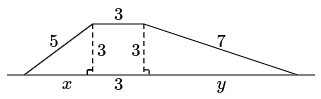
\includegraphics[width=0.4\textwidth]{../images/des_pitagoras_07.png}
    \end{center}
    \caption{}
    \label{fig:des_pitagoras_07}
\end{figure}

\textbf{¿Cuál es la distancia horizontal desde la posición inicial hasta la posición final del avión?}
\textit{Redondea tu respuesta a la décima de kilómetro más cercana.}
